\documentclass[t, 10pt]{beamer}
%%\documentclass[t,handout]{beamer}

\usepackage{graphicx}
\usepackage{epsfig}
\usepackage{psfrag}
\usepackage[english]{babel}
\usepackage{color}
%Mathematics packages
\usepackage{amsmath}
\usepackage{mathrsfs}
\usepackage{amsfonts}

\usepackage{enumerate}


\graphicspath{{./images/}} % Figures path - used in graphicx

\selectcolormodel{cmyk}

\mode<presentation>

%THEMES - Please refer to these chapters in the beamer documentation.
% Presentation themes : Chapter 15
% Color themes : Chapter 17
% Font themes : Chapter 18


\usetheme{Pittsburgh}
\usecolortheme{orchid}
\usefonttheme{default}

%---------------------------Title frame definition------------------------------------- 

\title{An Interoperable Framework for Usage Managment}
\author [Chris]{Christopher Lamb, Pramod Jamkhedkar, and Gregory Heileman}
\institute[University of New Mexico]{
\inst {}Department of Electrical and Computer Engineering\\
University of New Mexico}
\date{October 4, 2010}
\titlegraphic{
\begin{figure} 

\includegraphics[width = 7cm]{UNM}
\end{figure}}

% Delete this, if you do not want the table of contents to pop up at
% the beginning of each subsection:
%\AtBeginSubsection[]
%{
%  \begin{frame}<beamer>
%    \frametitle{Outline}
%     \tableofcontents[currentsection,currentsubsection]
%  \end{frame}
%}


\begin{document}

\begin{frame}
\titlepage
\end{frame}

% This command will make the logo appear on all frames excluding the title frame.
\logo {
\includegraphics[width = 2.5cm]{UNM}}

\begin{frame}
\frametitle{Outline}
\tableofcontents 
\end{frame}

\section{what we do}
\begin{frame}
\frametitle{what we do}
\begin{itemize}
\item \textit{UNM Informatics}: Information security, theory, and architectures this work is specific to information security 
\pause
\item \textit{Usage Management}: Control of how an artifact is used, covering everything \textit{after} access
\end{itemize}
\pause
Some quick definitions:
\begin{itemize}
\item \textit{PMR}: Personal medical record; in this case, this record is electronic
\item \textit{UM}: Usage management
\end{itemize}
\end{frame}

\section{applied to PMR}
\begin{frame}
\frametitle{um and pmr}

We believe PMRs have certain attributes that aren't addressed well by current management systems:
\pause
\begin{itemize}
\item \textit{Mashable}
\pause
\item \textit{Controllable}
\pause
\item \textit{Available}
\end{itemize}
\pause

Usage Management of PMRs enables these things, providing fine-grained management of \textit{information contained in PMRs}
\newline
\newline
\pause

This opens new business models:
\pause
\begin{itemize}
\item \textit{Remote Access}
\pause
\item \textit{Monitoring}
\pause
\item \textit{Custom Care}
\pause
\item \textit{Data Marketplace}
\pause
\end{itemize}
 
\end{frame}

\section{um primer}
\begin{frame}
\frametitle{um primer - system overview}
\pause

Three basic things:
\begin{figure}
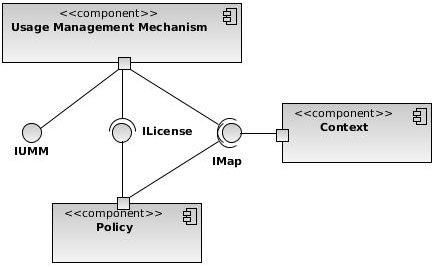
\includegraphics[width = 6cm]{Integrated}
\end{figure}

\begin{itemize}
\item \textit{Usage Management Mechanism}
\item \textit{Policy}
\item \textit{Context}
\end{itemize}
\pause

\end{frame}

\begin{frame}
\frametitle{um primer - ontology}

Ontology of domain required to pull it all together
\begin{figure}
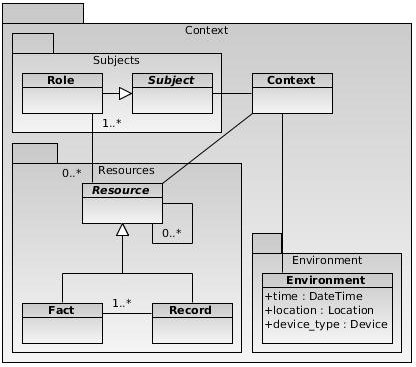
\includegraphics[width = 6cm]{UMOntology}
\end{figure}

\end{frame}

\begin{frame}
\frametitle{Assumptions}

\begin{itemize}
	\item Information ecosystems will operate across highly networked,
distributed, diverse computing environments.
\pause
	\item Resources will move across these computing environments
as well as different information ecosystems.
\pause
	\item Multiple information ecosystems will continue to use different
policy languages, depending on the types of rules and
rights models required for expressing their respective policies.
\pause
	\item No single policy language will be able address the policy expression
requirements of different information ecosystems.
Policy languages will continue to change and evolve using
different logics to express various usage semantics.
\end{itemize}

\end{frame}

%\bibliographystyle{plain}
%\bibliography{drm}

\end{document}

